\subsection{Zcash}

Zerocash \cite{Zerocash} is a novel proposal for a cryptographic protocol that addresses the inherent privacy limitations of bitcoin. It introduces the concept of decentralized anonymous payment (DAP) scheme, meaning a digital currency system where all transactions are guaranteed to be completely anonymous. That is, the origin, destination, and amount are all hidden from the public ledger.

Zerocash achieves privacy through the use of Zero-Knowledge Succinct, Non-interactive Arguments of Knowledge (zk-SNARKs). This cryptographic tool is essential to prove that transactions are valid, without revealing any information about the parties involved in a transaction and the amounts involved. 

More specifically, Zerocash functions on top of any ledger-based currency (e.g. Bitcoin). First, each user generates an arbitrary number of address key pairs. These contain a public key $\pk$ that allows others to send payments to the user, and a secret key $\sk$ that is used to receive payments sent to the corresponding public key. Then Zerocash gives the ability to users to convert  regular coins into anonymous coins through the mint functionality. Afterwards, users can spend (move) this coins in transactions without revealing any information. 

\subsubsection{Mint coins}
When minting a coin, a user generates a secret trapdoor $\rho$, used to create a random serial number unique for each coin (through a PRF) and two randomnesses $r, s$. Then they create a commitment to the value of the coin, the recipient's address and the serial number in the two following steps. First, user computes an intermediate commitment $k$ using randomness $r$ for the concatenation of the recipient address and the trapdoor $\rho$, $k = \com(\pk||\rho ; r)$. In the second step user creates a commitment using randomness $s$ for the concatenation of the coin's value and the intermediate commitment $k$, $cm = \com(\v||k;s)$.
Finally the user publish on the blockchain the mint transaction $\txn_{MINT} = (\v, k, s, cm)$. 

Anyone can verify that $cm$ is a commitment to a coin of value $v$ by checking whether $\com(\v||k;s)$ is equal to $cm$. However, they will not be able to distinguish between the owner $\pk$ and the serial number, since these values are hidden inside the commitment $k$.

All of the minted coins are stored in a "shielded pool" and are not deleted when spend in order to provide anonymity.

\subsubsection{Pour coins (Spend functionality)}

In order to spend a coin anonymously, the user produces a zero-knowledge proof (using zk-SNARK) for the statement:
"I know the one opening ($\rho, r)$ of a coin commitment of the "shielded pool" and the corresponding secret key $\sk$ such that $k = \com(\pk||\rho ; r)$ and $sn = PRF(\sk, \rho)$.

After that user reveal the serial number $sn$. The serial number is used in order to handle double spending. Zerocash allocates a unique sequence number to each coin, which is published on-chain when the coin is spent. Therefore, an attempt at double spending is indicated by a new transaction that produces a sequence number(s) that has already been published.

Finally, user creates a new coin for the new recipient address with a new serial number.

After confirming and recording the pour transaction in the ledger, the new coins can be used for future transactions. Throughout this process, the use of zk-SNARKs and commitments guarantees that all details of the transaction, including the coin spent and the recipient of the new coin, remain private and secure. This process maintains user anonymity while preserving the integrity and validity of transactions within the Zerocash system.

\subsubsection{Merkle Tree}
As mentioned above, to ensure anonymity, no one can tell which coin was used in each transaction. 
Thus, the spent coins cannot be removed from the "shielded pool". As a result, its size increases with each transaction. Therefore, the naive approach to implement it as a list of coin commitments will lead to a linear growth for the blockchain size. 

A more efficient implementation is the use of Merkle trees. 
Zerocash maintains an efficiently updateable Merkle tree over the growing coin commitment list \autoref{fig:zcash-merkle}. As a result, the space complexity is reduced to logarithmic.

\begin{figure}
    \centering
    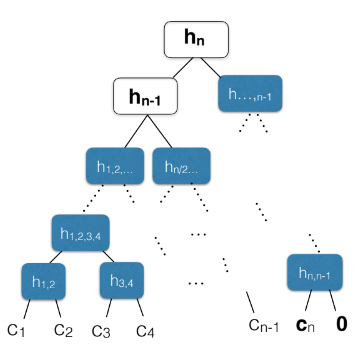
\includegraphics[width=0.8\textwidth]{images/zcash/merkle tree.png}
    \caption{Zerocash Merkle Tree of Coin Commitments}
    \label{fig:zcash-merkle}
\end{figure}

